\documentclass[withoutpreface]{cumcmthesis}

\begin{document}

\begin{abstractpage}{相关系数分析及其显著性检验}

    本文主要研究相关系数分析的作用和步骤。

    首先,我们引入了相关系数的概念,并从整体上认识了\textbf{ Pearson 相关系数}、 \textbf{Spearman 相关系数}和 \textbf{Kendall 相关系数}的异同。其次,我们又介绍了\textbf{描述性统计}的作用和意义。随后,我们分别详细介绍了三大相关系数的计算及其\textbf{显著性检验}。最后,以中学考试成绩的数据为例,我们进行了相关系数分析,展示和总结了前文介绍的分析流程。

    \keywords{线性相关 \quad 显著性检验 \quad 置信区间 \quad Pearson 相关系数 \quad Spearman 相关系数}
\end{abstractpage}

\tocpage

\section{相关系数简介}

两组数据之间,常常会显现出一种\textbf{线性相关性}。笼统地讲,数据列 A 的值上升,数据列 B 的值整体随之上升,称 A 与 B \textbf{正相关};数据列 A 的值上升,数据列 B 的值反而整体下降,称 A 与 B \textbf{负相关};数据列 A 的值上升,数据列 B 的值整体没有明显的上升或下降趋势,称 A 与 B \textbf{不相关}。

特别地,若数据列 A 、 B 的值符合一条斜率为正的直线,称 A 与 B \textbf{完全正相关};若数据列 A 、 B 的值符合一条斜率为负的直线,称 A 与 B \textbf{完全负相关}。

\begin{figure}[H]
    \centering
    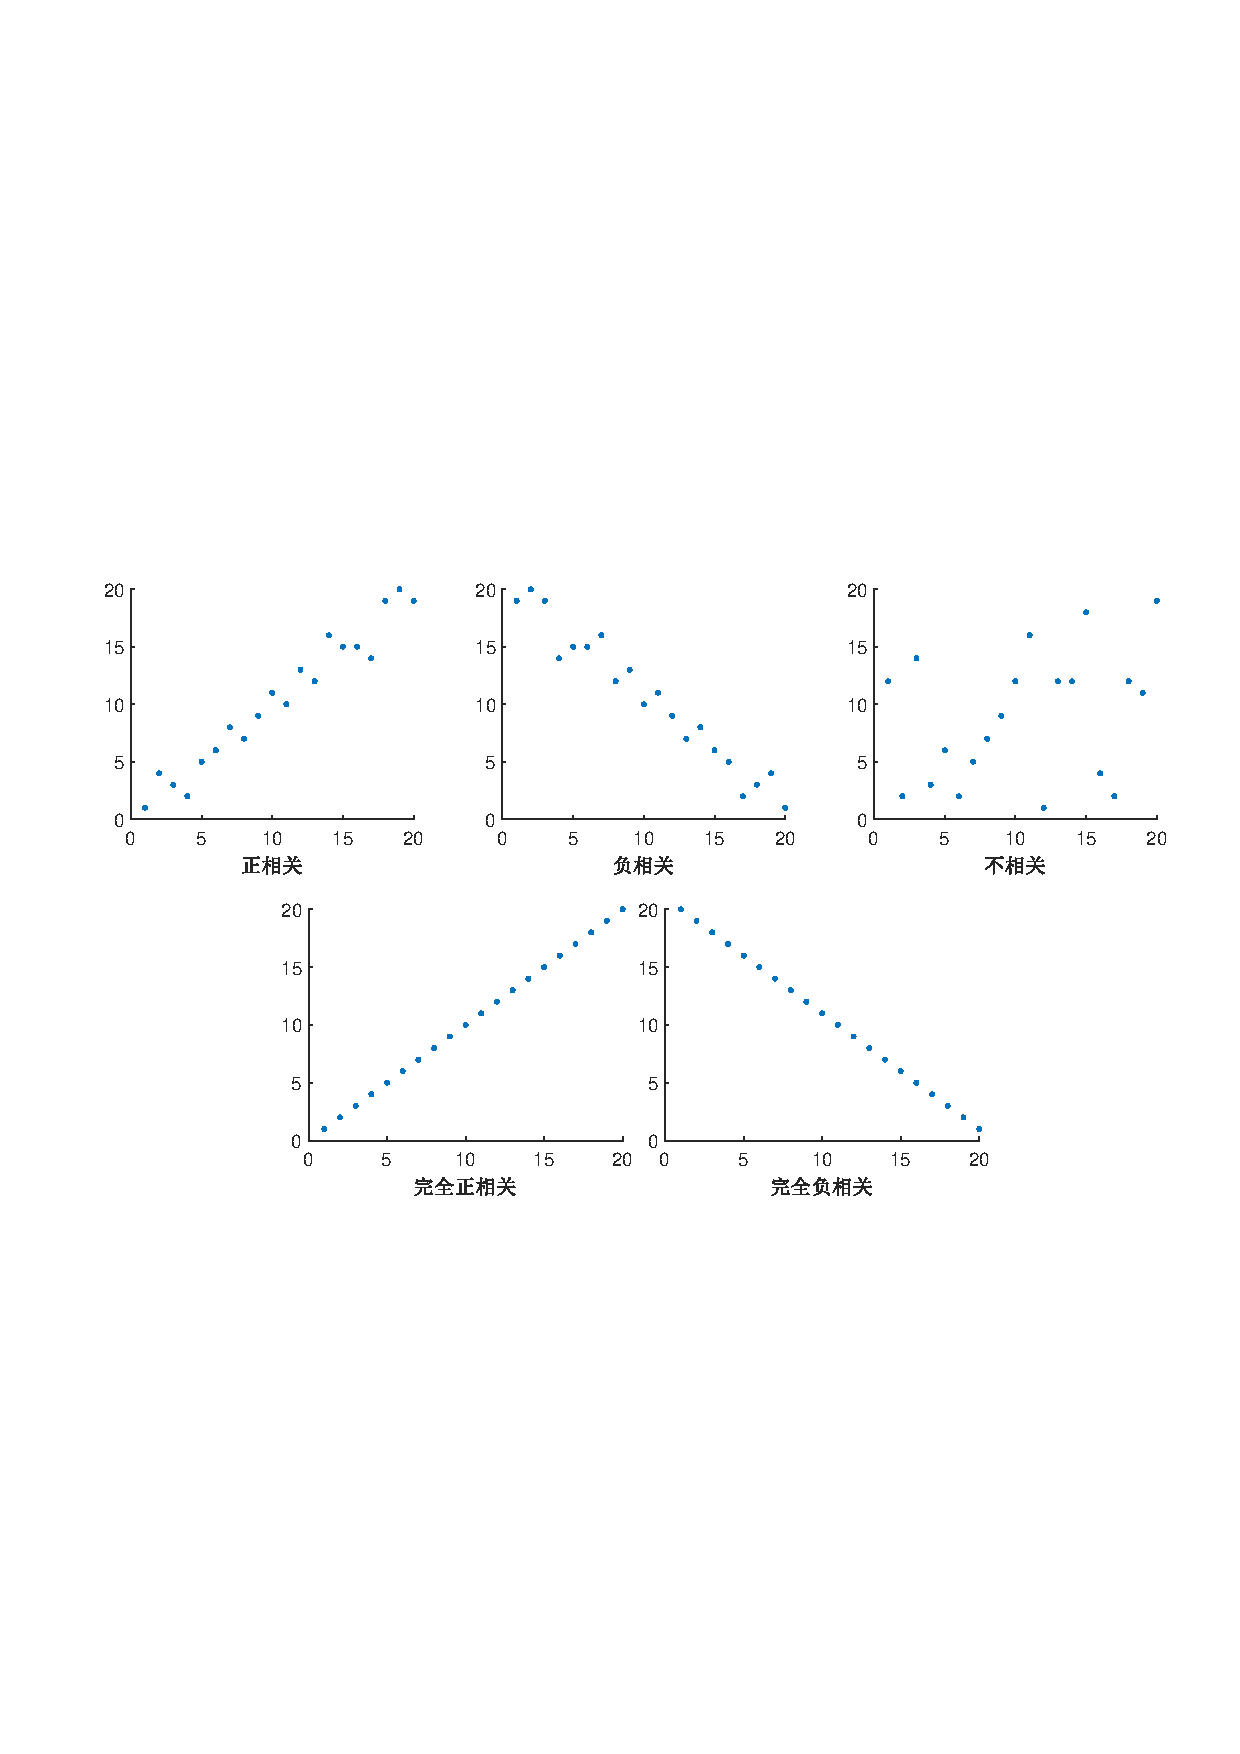
\includegraphics[width=0.9\textwidth]{线性相关}
    \caption{线性相关关系图示}\label{Fig:1}
\end{figure}

相关系数$r$是这样一个数值,它能在一定程度上衡量两组数据间的\textbf{线性相关性的大小},并且具有以下性质:

\begin{enumerate}
    \item $-1\le r \le1$
    \item $r=1$ 时,两组数据完全正相关;$r=-1$ 时,两组数据完全负相关;$r=0$时,两组数据明显不具有线性相关性。
    \item $|r|$越大,两组数据的线性相关性越强;正负符号代表正负相关
\end{enumerate}

常见的相关系数有三种: Pearson 相关系数、 Spearman 相关系数、 Kendall 相关系数。

\begin{table}[H]
    \centering
    \begin{tabular}{cc}
        \toprule[1.5pt]
        \makebox[0.1\textwidth][c]{相关系数} & \makebox[0.8\textwidth][c]{要求}                     \\
        \midrule
        $Pearson$                        & 无明显异常值;数据为连续变量;两组数据呈\textbf{正态分布}或\textbf{近似正态分布}; \\
        $Spearman$                       & 对数据无特殊要求                                           \\
        $Kendall$                        & 两组数据中包含\textbf{定序变量};对数据分布无特殊要求                    \\
        \bottomrule[1.5pt]
    \end{tabular}
\end{table}

\section{描述性统计及线性关系检测}

在对数据进行线性相关性分析之前,我们可以先进行描述性统计,以对数据有一个整体的认识。

假设进行统计性描述的数据列为$X$,则常见的统计量有
\begin{equation*}
    \mbox{最大值:} \max(X) = \max\{x_1,x_2,\cdots,x_n\}
\end{equation*}
\begin{equation*}
    \mbox{最小值:} \max(X) = \min\{x_1,x_2,\cdots,x_n\}
\end{equation*}
\begin{equation*}
    \mbox{中位数:} m_{0.5}(X) = [(X)_{sorted}]_{median}
\end{equation*}
\begin{equation*}
    \mbox{平均值:} \mu(X) = \frac{\sum\limits_{i=1}^{n}x_i}{n}
\end{equation*}
\begin{equation*}
    \mbox{标准差:} \sigma(X) = \sqrt{\frac{\sum\limits_{i=1}^{n}(x_i - \mu)^2}{n-1}}
\end{equation*}
\begin{equation*}
    \mbox{峰度:} Kurt(X) = \frac{\frac{1}{n}\sum\limits_{i=1}^{n}(x_i-\mu)^4}{[\frac{1}{n}\sum\limits_{i=1}^{n} (x_i-\mu)^2]^2}-3
\end{equation*}
\begin{equation*}
    \mbox{偏度:} Skew(X) =  \frac{\frac{1}{n}\sum\limits_{i=1}^{n}(x_i-\mu)^3}{[\frac{1}{n}\sum\limits_{i=1}^{n} (x_i-\mu)^2]^{\frac{3}{2}}}
\end{equation*}

其中,峰度和偏度的绝对值越接近0,可以初步认为数据的分布越接近于正态分布。

除了描述性统计,我们还需要绘制出想要分析的两组数据对应的散点图,查看它们是否具有一定的线性相关关系。如果数据符合的是\textbf{很明显的非线性关系},那我们就要尽早放弃使用线性相关系数分析方法了。

\section{Pearson 相关系数}
\subsection{正态性检验}
在进行 Pearson 相关系数的计算之前,首先要检验数据的正态性。方法有很多:需要大量数据的 Q-Q 图法、大样本 (n>30) 的 Jarque-Bera 检验、小样本 ($3 \le n \le 50$) 的 Shapiro-wilk 检验。

\subsubsection{Q-Q 图}

分位图 (quantile-quantile plot) ,又称 Q-Q 图,通过比较两组数据的分位数,来判断两者是否同分布。令其中一组数据为标准正态分布 $N(0,1)$,另一组为标准化后的已知数据,这样就能够判断已知数据是否具有一定的正态性了。

\begin{figure}[H]
    \centering
    \includegraphics[width=0.9\textwidth]{qq图}
    \caption{Q-Q 图示意}\label{Fig:2}
\end{figure}

如\cref{Fig:2}所示,如果 Q-Q 图接近于一条直线(左),可以认为数据具有较好的正态性;否则,与一条直线有较大偏差(右),可以认为数据的正态性较差。

值得注意的是,只有数据量较大时, Q-Q 图的效果才会很明显。

\subsubsection{Jarque-Bera 检验}

当$n\ge 30$时,可以进行 Jarque-Bera 检验。

在描述性统计中,得到的峰度 (K) 和 偏度 (S) 已经能够初步检测数据的正态性了。不过为了更加准确,我们可以通过峰度和偏度构造一个新的统计量——— JB 统计量。
\begin{equation}\label{Eq:1}
    \mbox{JB 统计量:}  JB = \frac{n}{6}(S^2+\frac{K^2}{4})
\end{equation}

经过证明,如果数据服从正态分布,那么对应的 JB 统计量将近似服从自由度为2的 $\chi^2$ 分布。
\begin{equation}
    \mbox{自由度为2的$\chi^2$分布的概率密度函数:} f(y) = \begin{cases}
        \frac{1}{2\Gamma(1)} e^{-\frac{y}{2}} & y>0    \\
        0                                     & y\le 0
    \end{cases}
    \label{Eq:2}
\end{equation}

据此,我们可以根据由数据计算出来的$JB^*$对数据的正态性进行假设检验。具体步骤如下:

\begin{enumerate}
    \item \textbf{作出假设}。原假设$H_0$为“已知数据服从正态分布”,备选假设$H_1$为“已知数据不服从正态分布”。
    \item \textbf{计算}$\mathbf{JB^*}$。先计算峰度 (K) 和 偏度 (S),再进一步通过\cref{Eq:1}计算$JB^*$
    \item \textbf{计算 p 值}。 根据概率密度函数\cref{Eq:2}或其他手段计算出$JB\ge JB^*$的概率,即p值(此处为单侧检验)。
    \item \textbf{选择显著性水平}$\mathbf{\alpha}$。$p<\alpha$代表在$(1-\alpha)\times 100\%$的置信水平上拒绝原假设。常见的是$\alpha=0.05$。
    \item \textbf{得出结论}。若拒绝原假设,说明数据并不服从近似的正态分布。
\end{enumerate}

\begin{figure}[H]
    \centering
    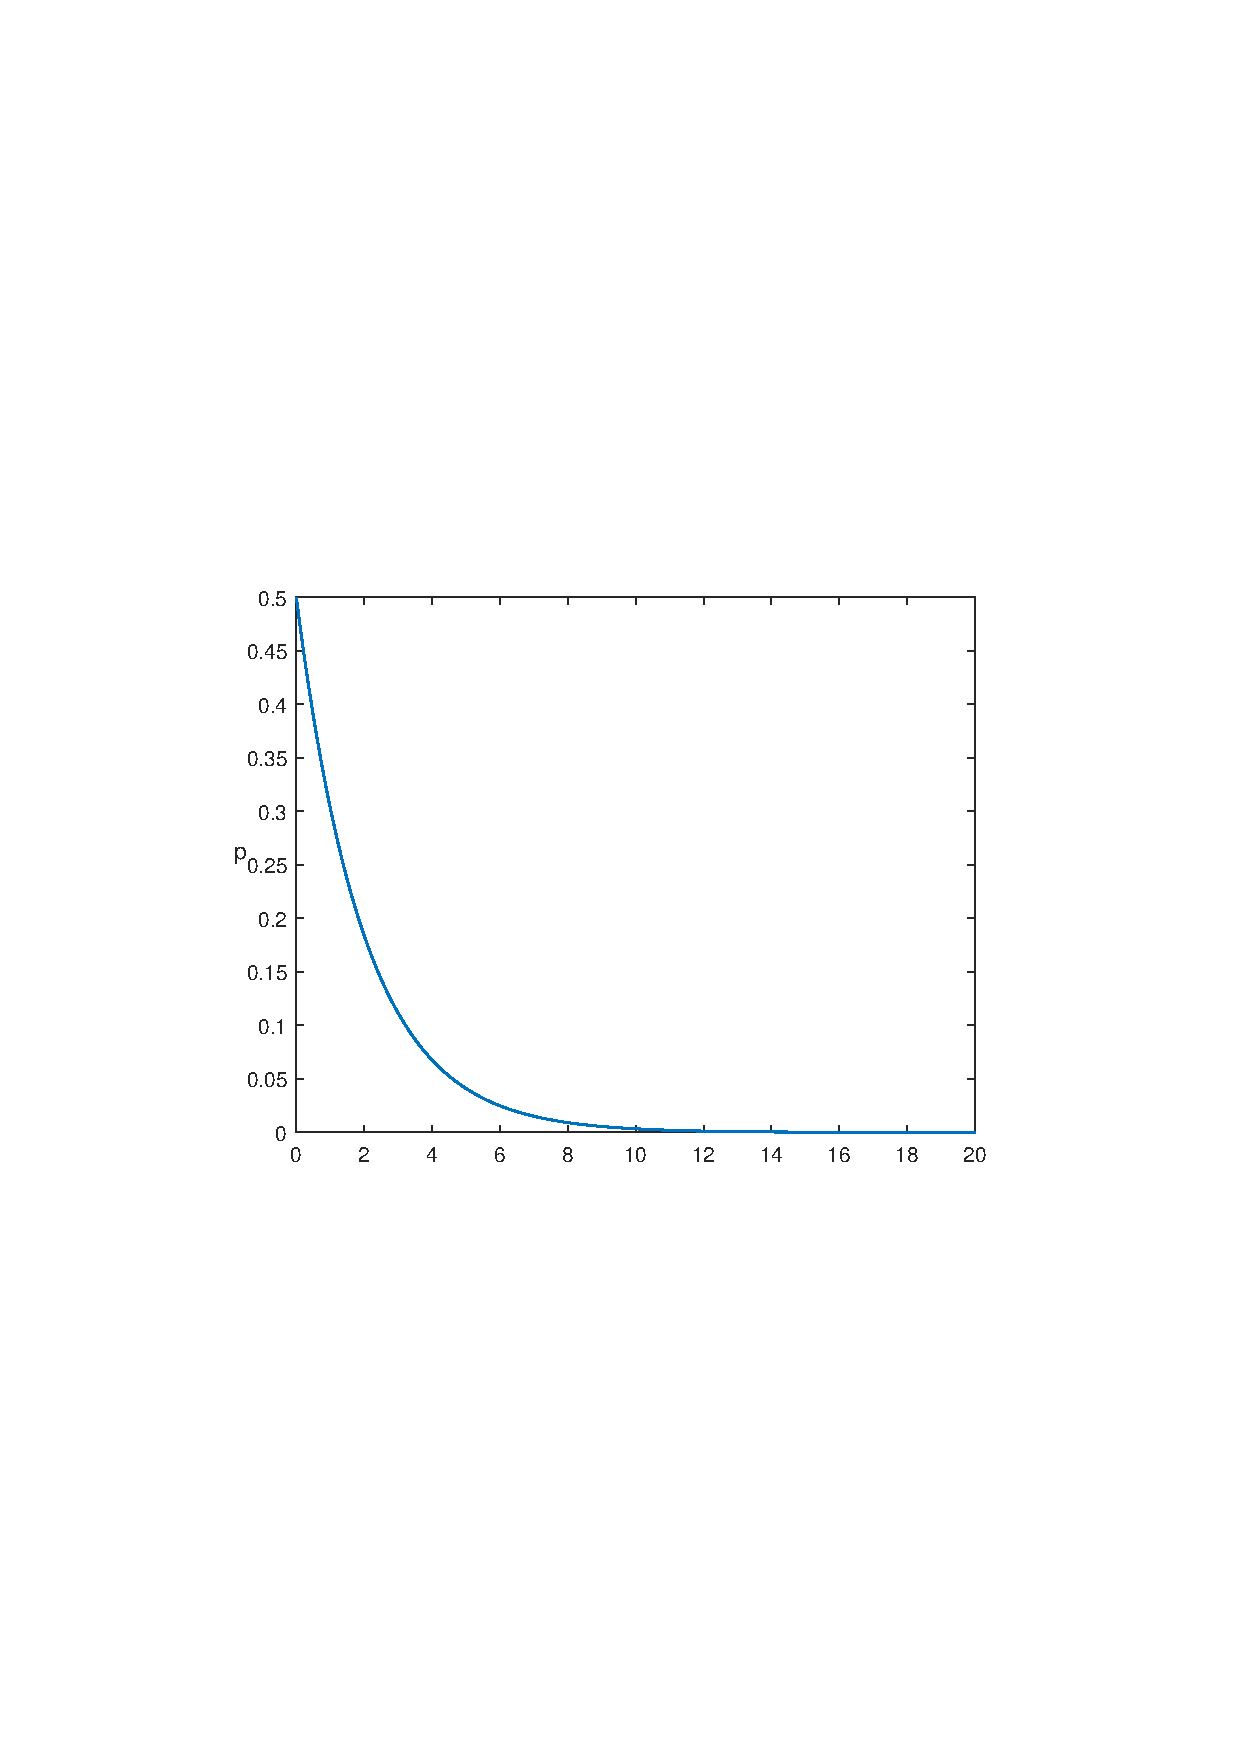
\includegraphics[width=0.7\textwidth]{自由度为2的卡方分布}
    \caption{自由度为2的卡方分布的概率密度函数图像}\label{Fig:3}
\end{figure}

\subsubsection{Shapiro-wilk 检验}

当$3\le n \le 50$时,可以进行Shapiro-wilk 检验。

和 Jarque-Bera 检验类似,构造统计量$W$,则$W$将服从一个已知分布(尚未命名)。据此进行假设检验。

\begin{equation}
    W = \frac{(\sum\limits_{i=1}^{n} a_ix_i)^2}{\sum\limits_{i=1}^{n} (x_i-\mu)^2}
\end{equation}

具体步骤为:
\begin{enumerate}
    \item \textbf{作出假设}。原假设$H_0$为“已知数据服从正态分布”,备选假设$H_1$为“已知数据不服从正态分布”。
    \item \textbf{计算}$\mathbf{W}$。
    \item \textbf{计算 p 值}。通过已有实现计算出 p 值。
    \item \textbf{选择显著性水平}$\mathbf{\alpha}$。$p<\alpha$代表在$(1-\alpha)\times 100\%$的置信水平上拒绝原假设。常见的是$\alpha=0.05$。
    \item \textbf{得出结论}。若拒绝原假设,说明数据并不服从近似的正态分布。
\end{enumerate}

\subsection{相关系数计算}

Pearson 相关系数基于协方差推导而来。
\begin{equation}
    \mbox{协方差} Cov(X,Y) = \frac{\sum\limits_{i=1}^{n} (x_i-\bar x)(y_i-\bar y)}{n-1}
\end{equation}

协方差初步体现了数据$X,Y$之间的线性相关性:若$Cov(X,Y)$大于0,说明$(x_i-\bar x)$和$(y_i-\bar y)$整体符号相同,也就是 X 和 Y 的变化趋势大致相同。

协方差受量纲影响较大,将协方差标准化,就可以得到 Pearson 相关系数。
\begin{equation}
    r = \frac{Cov(X,Y)}{\sigma_X\sigma_Y} = \frac{\sum\limits_{i=1}^{n} (x_i-\bar x)(y_i-\bar y)}{\sqrt{\sum\limits_{i=1}^{n}(x_i - \bar x)^2} \sqrt{\sum\limits_{i=1}^{n}(y_i - \bar y)^2}}
\end{equation}

\subsection{显著性检验}

有时候由于数据量大和异常值等其他原因,导致相关系数较小。我们可以通过假设检验来判断相关系数是否显著不等于0,从而说明两组数据间确实存在线性相关性。通常使用 t 检验。

由 Pearson 相关系数$r$构造$t$统计量,经证明,$t$将服从自由度为$n-2$的$t$分布。
\begin{equation}\label{Eq:6}
    t = r\sqrt{\frac{n-2}{1-r^2}}
\end{equation}
\begin{equation}\label{Eq:7}
    \mbox{自由度为$n$的$t$分布的概率密度函数:}f(x)=\frac{\Gamma(\frac{n+1}{2})}{\sqrt{\pi n}\Gamma(\frac{n}{2})}(1+\frac{x^2}{n})^{-\frac{n+1}{2}}
\end{equation}

\begin{figure}[H]
    \centering
    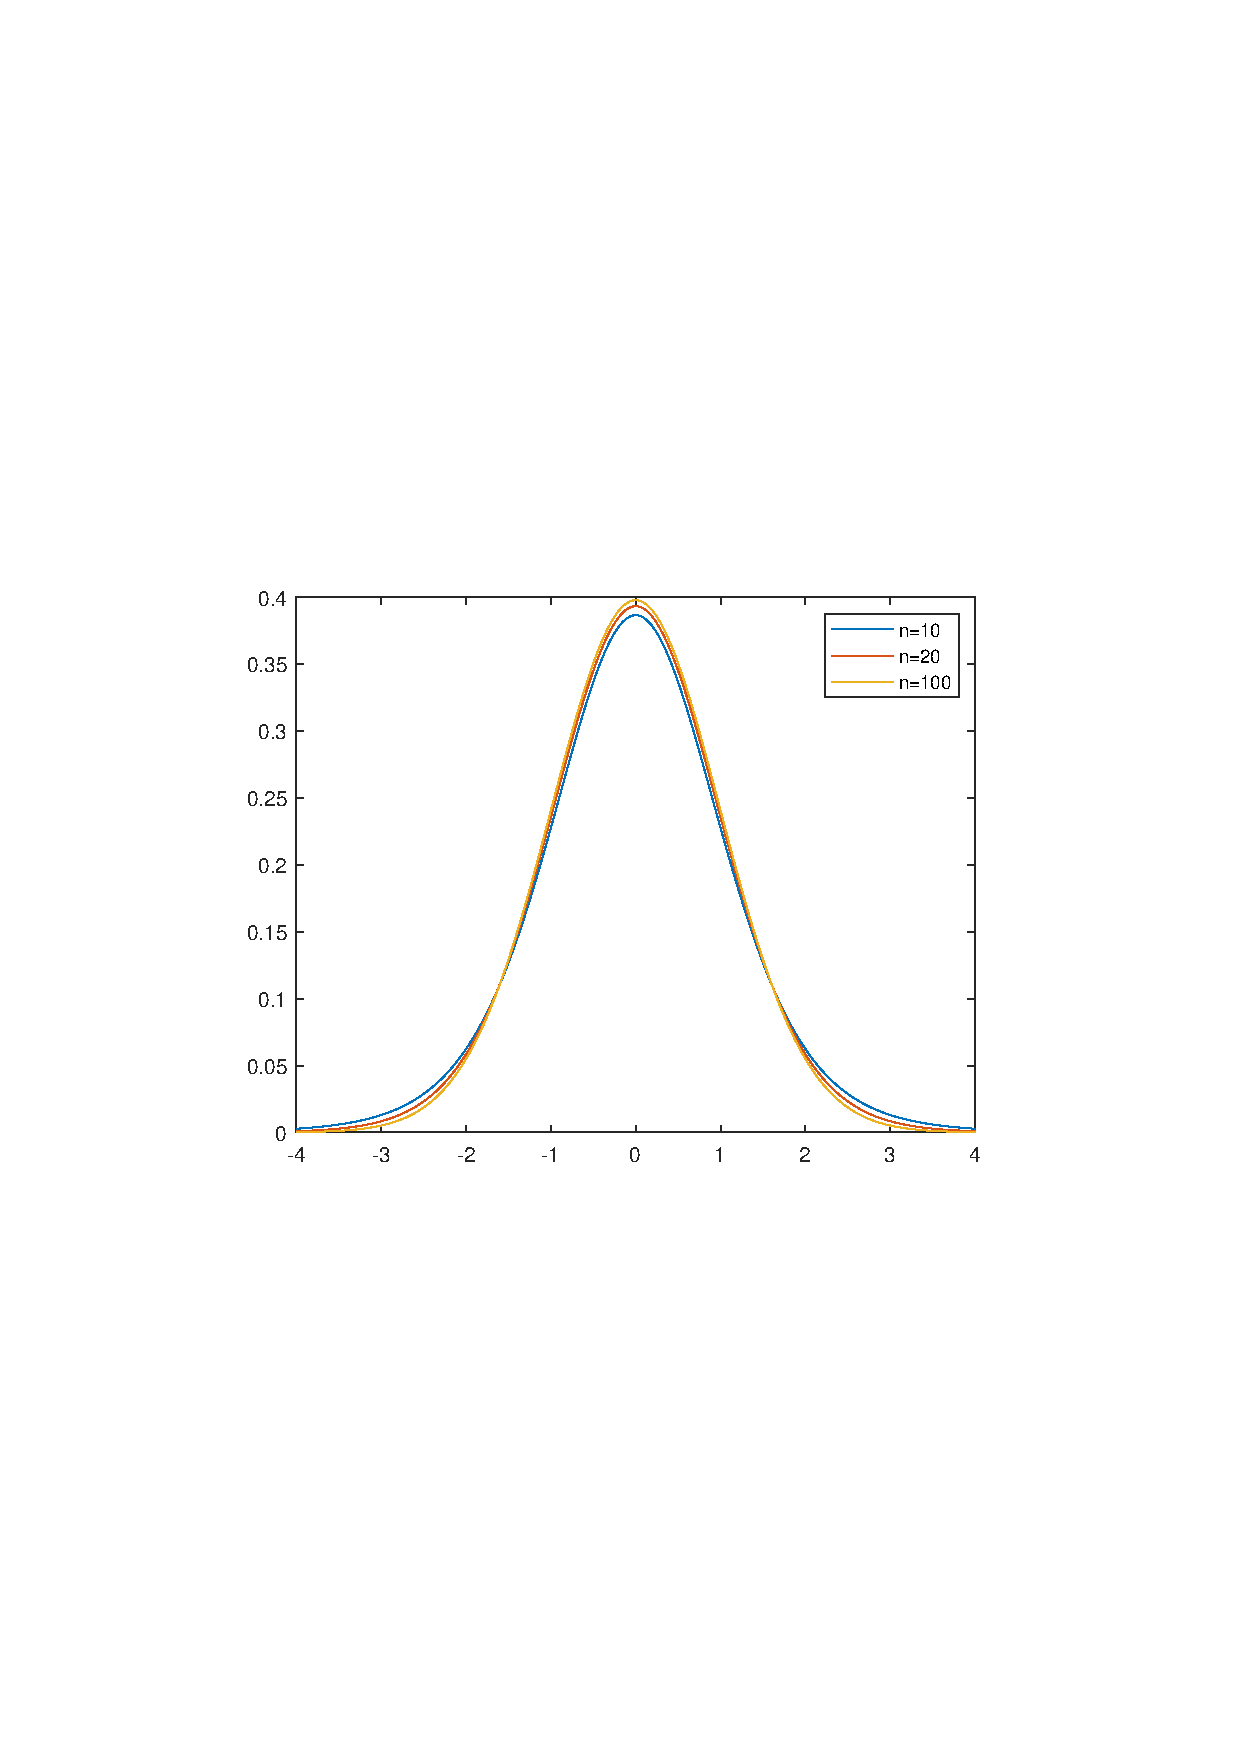
\includegraphics[width=0.46\textwidth]{t分布}
    \caption{t 分布概率密度函数图像}\label{Fig:4}
\end{figure}

t 检验具体步骤如下:

\begin{enumerate}
    \item \textbf{作出假设}。原假设$H_0$为“$r=0$”,备选假设$H_1$为“$r\ne 0$”。
    \item \textbf{计算}$\mathbf{t^*}$。通过\cref{Eq:6}计算$t^*$
    \item \textbf{计算 p 值}。 根据概率密度函数\cref{Eq:7}或其他手段计算出$|t|\ge |t^*|$的概率,即p值(此处为双侧检验)。
    \item \textbf{选择显著性水平}$\mathbf{\alpha}$。$p<\alpha$代表在$(1-\alpha)\times 100\%$的置信水平上拒绝原假设。常见的是$\alpha=0.1(*),0.05(**),0.01(***)$。
    \item \textbf{得出结论}。若拒绝原假设,说明$r$显著不为0,即数据间确实具有一定的线性相关性,相关性由$r$的大小展示。
\end{enumerate}

\section{Spearman 相关系数}

与 Pearson 相关系数相比, Spearman 相关系数对数据的要求较小。因此不满足 Pearson 相关系数的条件,均可以考虑使用 Spearman 相关系数进行分析。

\subsection{相关系数计算}

在进行 Spearman 相关系数计算之前,要先把两组数据分别从小到大排序,得到对应的秩(即排名),再计算每一对数据对应的秩差$d_i$。

Spearman 相关系数有两种定义。两者计算出来的值略有差异。

第一种基于 Pearson 相关系数: Spearman 相关系数 是两组数据的秩的 Pearson 相关系数。

第二种基于秩差:
\begin{equation}
    r = 1-\frac{6 \sum\limits_{i=1}^{n} d_i^2}{n(n^2-1)}
\end{equation}

\subsection{显著性检验}

显著性检验与 Spearman 的 t 检验原理和步骤差不多。各统计软件和编程语言均有实现。不在此赘述。

\section{Kendall 相关系数}

Kendall 相关系数与 Spearman 相关系数类似,对数据的要求较小,通常用于分析定序数据。

\subsection{相关系数的计算}

Kendall 相关系数的计算与同序对数和异序对数有关。

如果两对数据的两个属性排序的方向相同,就称其为同序对。否则称为异序对。同序对和异序对对数和一般为$C_n^2=\frac{n(n-1)}{2}$对。将同序对数($n_c$)和异序($n_d$)之差与总对数之比定义为 Kendall 相关系数。
\begin{equation}
    r = \frac{2(n_c-n_d)}{n(n-1)}
\end{equation}

\subsection{显著性检验}

Kendall 相关系数的显著性检验较为复杂,各编程语言和统计软件均有实现,调用即可。

\section{实例}

\subsection{题目}
给出数据如\cref{Tab:1},请进行相关性分析。(仅作为示例,数据不一定准确)

\begin{table}[H]
    \centering
    \caption{示例数据}\label{Tab:1}
    \begin{tabular}{|c|c|c|c|c|c|c|}
        \hline
        语文     & 数学     & 英语     & 生物     & 历史     & 地理     & 政治           \\
        \hline
        80     & 92     & 98     & 79     & 76     & 87     & 78 \bigstrut \\
        \hline
        76     & 85     & 97     & 76     & 74     & 90     & 84 \bigstrut \\
        \hline
        88     & 84     & 90.5   & 67     & 62     & 68     & 78 \bigstrut \\
        \hline
        57     & 82     & 84.5   & 74     & 74     & 67     & 64 \bigstrut \\
        \hline
        69     & 72     & 83     & 63     & 50     & 85     & 57 \bigstrut \\
        \hline
        73     & 85     & 90     & 50     & 56     & 67     & 52 \bigstrut \\
        \hline
        66     & 81     & 84     & 59     & 56     & 61     & 61 \bigstrut \\
        \hline
        85     & 80     & 94     & 64     & 32     & 60     & 42 \bigstrut \\
        \hline
        69     & 77     & 80     & 50     & 38     & 60     & 72 \bigstrut \\
        \hline
        70     & 83     & 74.5   & 52     & 42     & 58     & 55 \bigstrut \\
        \hline
        72     & 82     & 77     & 59     & 40     & 66     & 33 \bigstrut \\
        \hline
        \vdots & \vdots & \vdots & \vdots & \vdots & \vdots & \vdots       \\
        \hline
    \end{tabular}
\end{table}

\subsection{描述性统计}

首先对数据进行描述性统计,结果如\cref{Tab:2}

\begin{table}[H]
    \centering
    \caption{描述性统计结果}\label{Tab:2}
    \begin{tabular}{|c|c|c|c|c|c|c|c|}
        \hline
            & 语文      & 数学      & 英语      & 生物      & 历史      & 地理      & 政治      \\
        \hline
        最大值 & 88      & 92      & 98      & 79      & 76      & 90      & 84      \\
        \hline
        最小值 & 4       & 9       & 25      & 12      & 8       & 14      & 6       \\
        \hline
        中位数 & 54.5    & 67.5    & 68.75   & 35.5    & 34      & 48.5    & 33.5    \\
        \hline
        平均值 & 52.7222 & 66.2778 & 65.7037 & 39.6296 & 35.7407 & 48.4444 & 35.0185 \\
        \hline
        标准差 & 18.8934 & 15.0087 & 20.4887 & 15.9401 & 16.1130 & 17.0423 & 19.1425 \\
        \hline
        峰度  & -0.4263 & 2.9542  & -0.9330 & -0.1939 & 0.2080  & -0.1923 & -0.0275 \\
        \hline
        偏度  & -0.3115 & -1.3363 & -0.2684 & 0.6684  & 0.7244  & 0.2576  & 0.6529  \\
        \hline
    \end{tabular}
\end{table}

紧接着绘制矩阵散点图,以整体观察数据间的相关情况。
\begin{figure}[H]
    \centering
    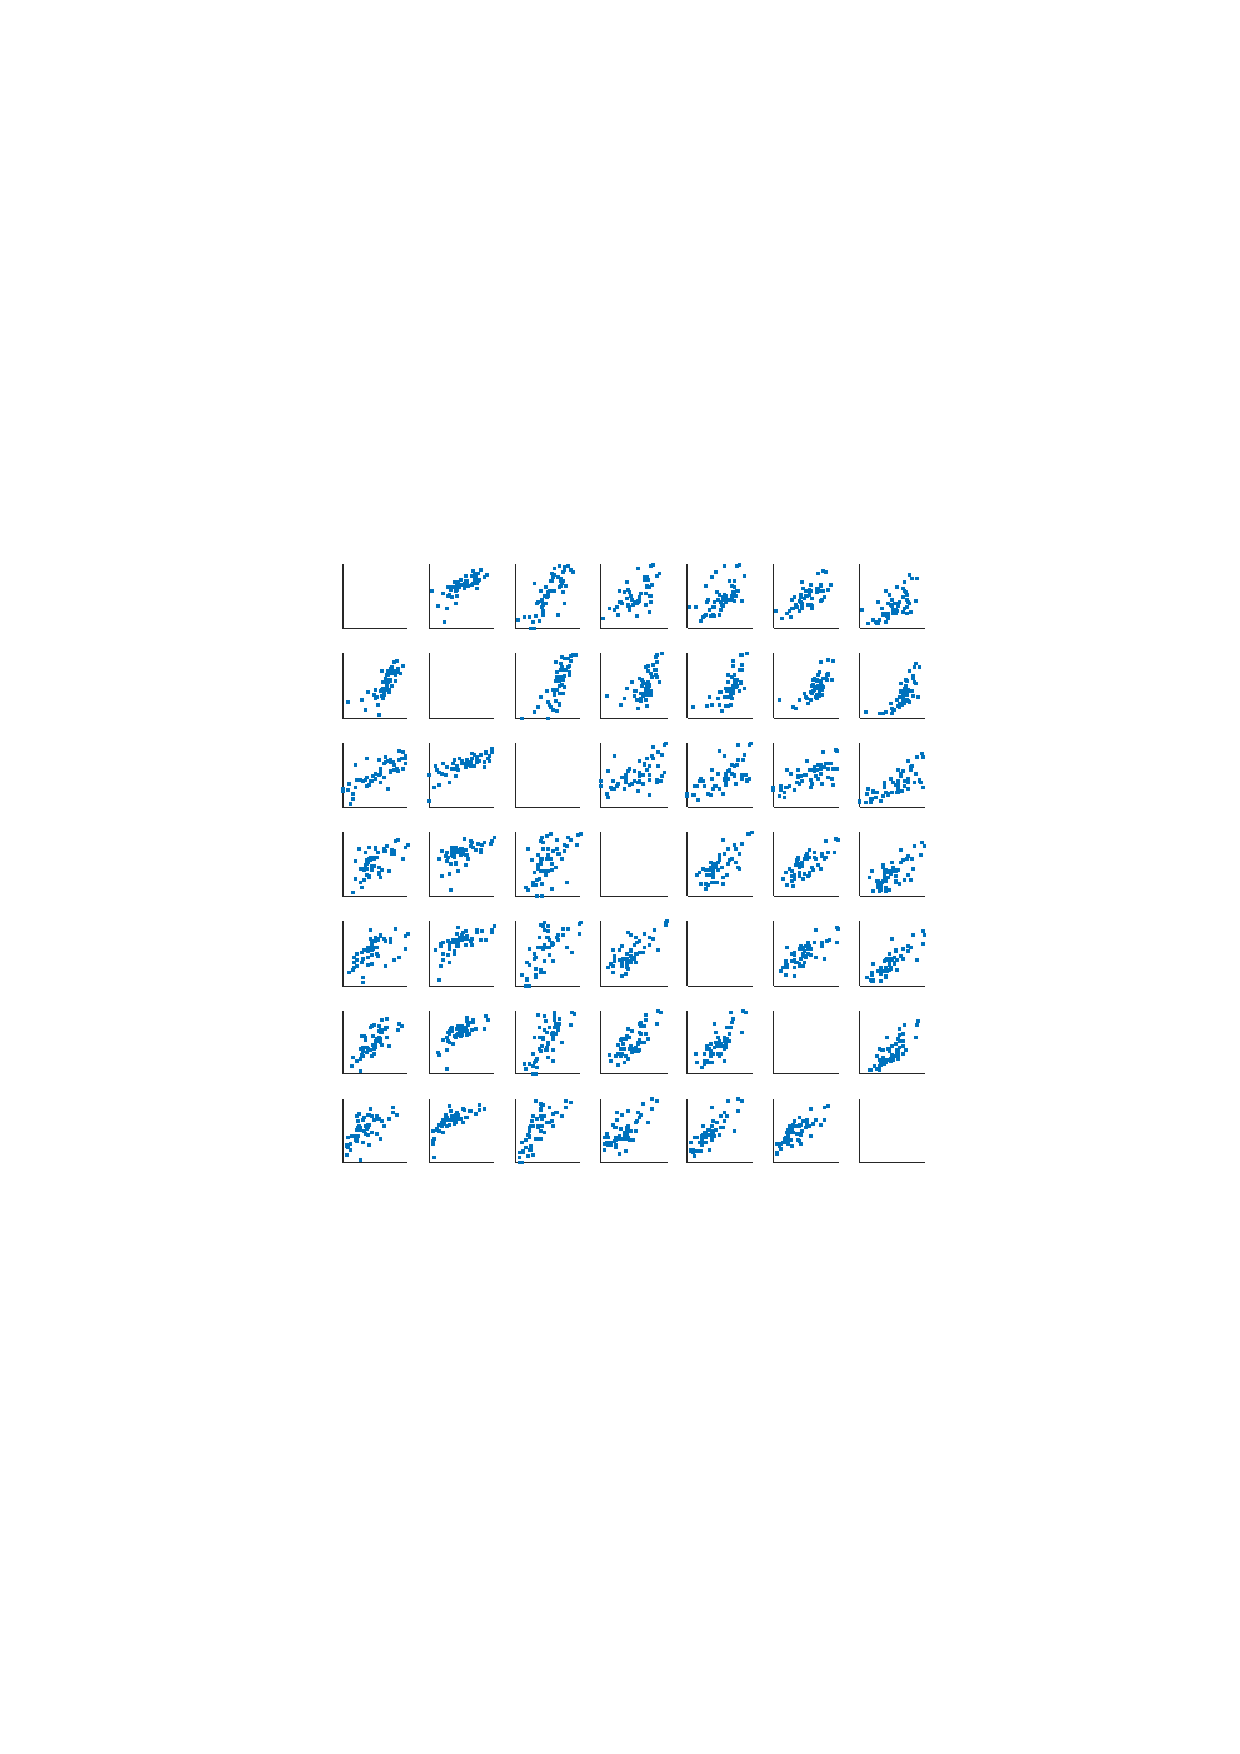
\includegraphics[width=0.6\textwidth]{散点图}
    \caption{矩阵散点图}\label{Fig:5}
\end{figure}
\subsection{Pearson 相关系数}

各数据列均为连续变量,符合 Pearson 相关系数的基本应用条件。

首先进行\textbf{正态性检验}。

绘制Q-Q图如\cref{Fig:6}。可以看出,各列数据 Q-Q 图都与直线有较好的拟合。在一定程度上,可以判断各列数据服从近似正态分布。

\begin{figure}[H]
    \centering
    \includegraphics[width=0.8\textwidth]{qq图2}
    \caption{各列数据对应的 Q-Q 图}\label{Fig:6}
\end{figure}

为了准确性,对各列数据进行 Shapiro-wilk 检验,得到如\cref{Tab:3}结果。除了语文和地理两列,其余各列都以90\% 及以上的置信水平服从正态分布。

\begin{table}[H]
    \centering
    \caption{Shapiro-wilk 检验结果}\label{Tab:3}
    \begin{tabular}{|c|c|c|c|c|c|c|c|}
        \hline
        学科    & 语文     & 数学     & 英语     & 生物     & 历史     & 地理     & 政治     \\
        \hline
        拒绝原假设 & 否      & 是      & 是      & 是      & 是      & 否      & 是      \\
        \hline
        p 值   & 0.5882 & 0.0007 & 0.0778 & 0.0294 & 0.0244 & 0.4242 & 0.0368 \\
        \hline
    \end{tabular}
\end{table}

为了保持研究的统一性,这里将语文和地理两列也视作近似服从正态分布进行处理。

接下来,两两计算 Spearman 相关系数并进行显著性检验,得到结果如\cref{Tab:4}。

为了直观性,绘制相关系数热力图如。

可以发现,各门学科之间的分数都具有很强的相关性,这说明大部分学生的各门分数都很均衡,相关性很强。尤其是语数英、政史地之间的的相关性极其突出。

\begin{table}[H]
    \centering
    \caption{Pearson 相关系数计算结果}\label{Tab:4}
    \begin{tabular}{|c|c|c|c|c|c|c|c|}
        \hline
           & 语文        & 数学        & 英语        & 生物        & 历史        & 地理        & 政治        \\
        \hline
        语文 & 1.00(***) & 0.75(***) & 0.77(***) & 0.60(***) & 0.56(***) & 0.71(***) & 0.64(***) \\
        \hline
        数学 & 0.75(***) & 1.00(***) & 0.77(***) & 0.59(***) & 0.68(***) & 0.73(***) & 0.73(***) \\
        \hline
        英语 & 0.77(***) & 0.77(***) & 1.00(***) & 0.55(***) & 0.65(***) & 0.69(***) & 0.75(***) \\
        \hline
        生物 & 0.60(***) & 0.59(***) & 0.55(***) & 1.00(***) & 0.74(***) & 0.71(***) & 0.70(***) \\
        \hline
        历史 & 0.56(***) & 0.68(***) & 0.65(***) & 0.74(***) & 1.00(***) & 0.76(***) & 0.84(***) \\
        \hline
        地理 & 0.71(***) & 0.73(***) & 0.69(***) & 0.71(***) & 0.76(***) & 1.00(***) & 0.78(***) \\
        \hline
        政治 & 0.64(***) & 0.73(***) & 0.75(***) & 0.70(***) & 0.84(***) & 0.78(***) & 1.00(***) \\
        \hline
    \end{tabular}

    \vspace{0.3cm}
    {\zihao{5}注:***、**、*分别代表1\%、5\%、10\%的显著性水平}
\end{table}

\begin{figure}[H]
    \centering
    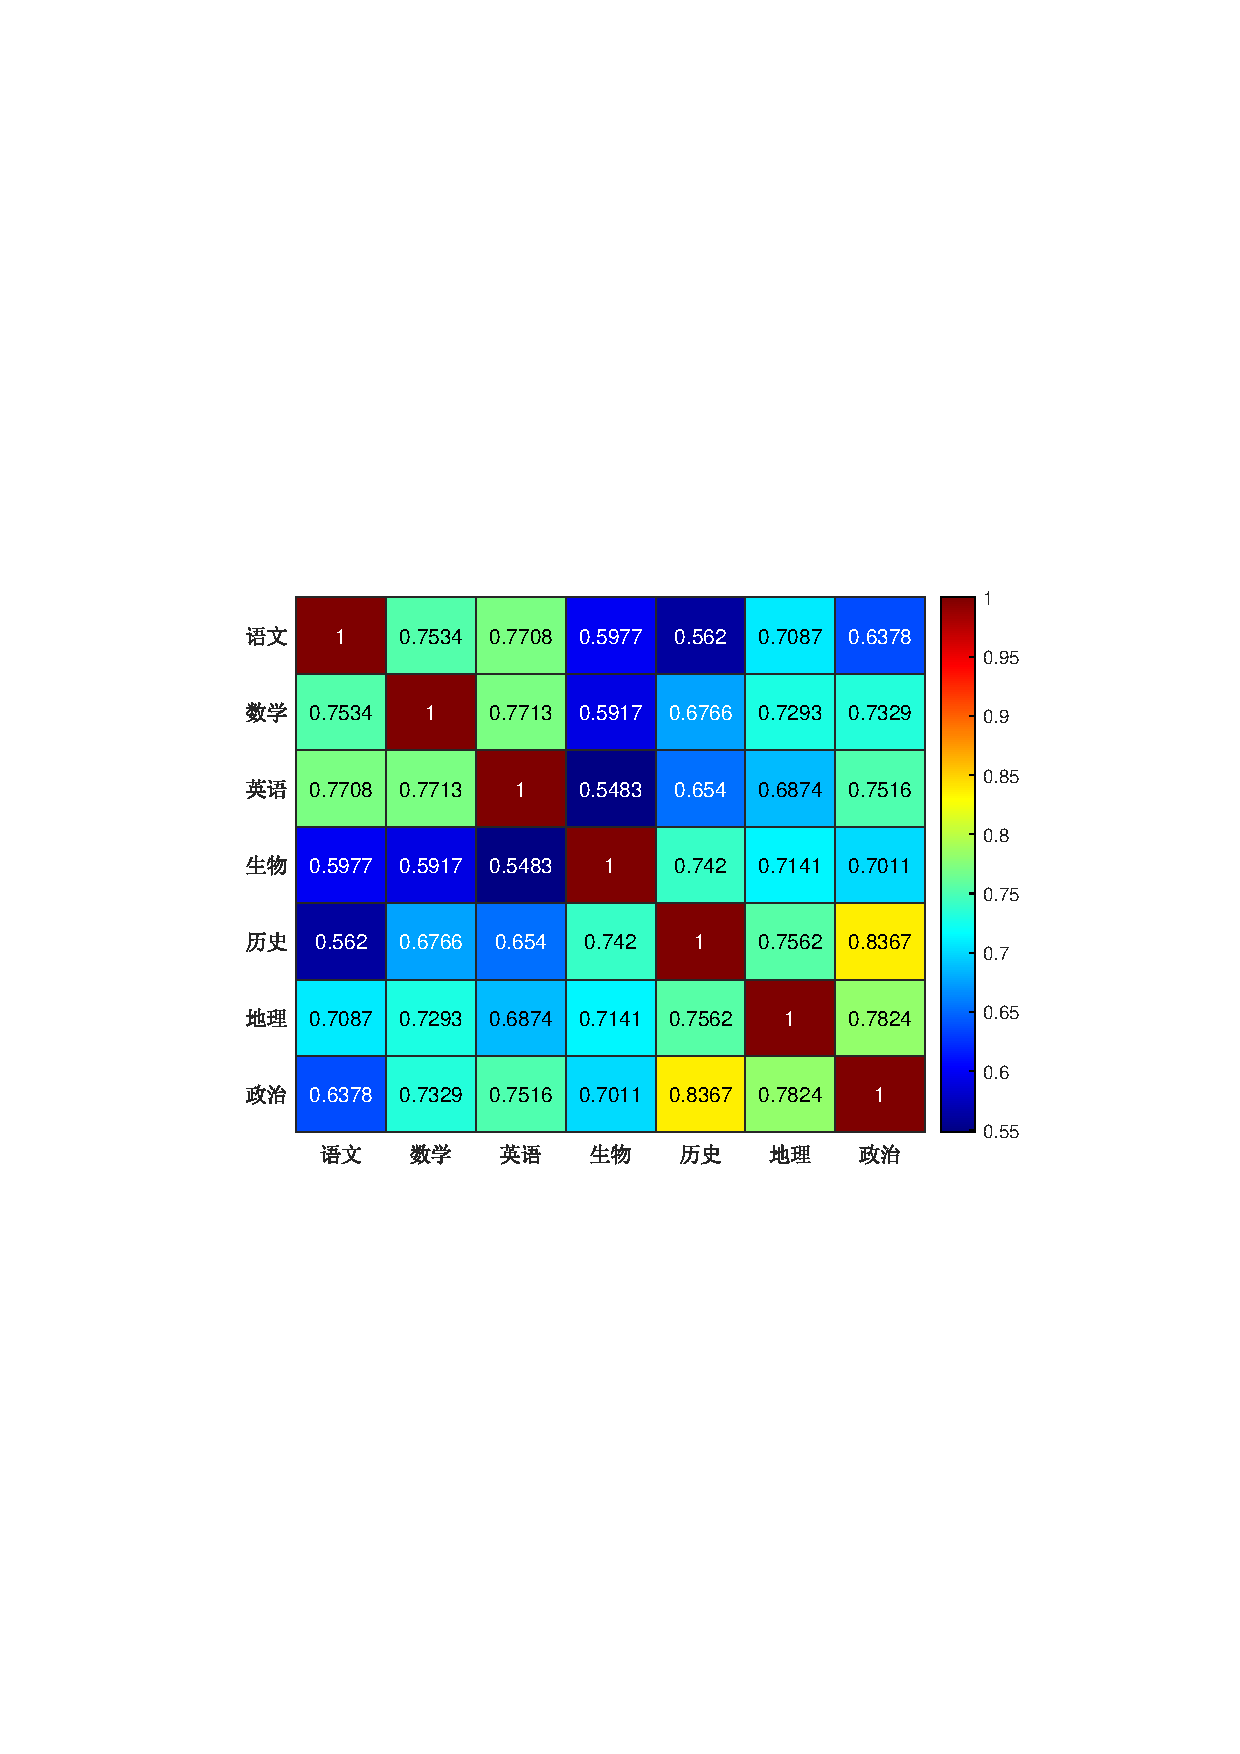
\includegraphics[width=0.8\textwidth]{相关系数热力图}
    \caption{Pearson 相关系数热力图}
\end{figure}

\subsection{Spearman 相关系数}

\begin{table}[H]
    \centering
    \caption{Kendall 相关系数计算结果}\label{Tab:6}
    \begin{tabular}{|c|c|c|c|c|c|c|c|}
        \hline
           & 语文        & 数学        & 英语        & 生物        & 历史        & 地理        & 政治        \\
        \hline
        语文 & 1.00(***) & 0.82(***) & 0.77(***) & 0.56(***) & 0.64(***) & 0.69(***) & 0.66(***) \\
        \hline
        数学 & 0.82(***) & 1.00(***) & 0.79(***) & 0.64(***) & 0.76(***) & 0.74(***) & 0.77(***) \\
        \hline
        英语 & 0.77(***) & 0.79(***) & 1.00(***) & 0.56(***) & 0.68(***) & 0.68(***) & 0.78(***) \\
        \hline
        生物 & 0.56(***) & 0.64(***) & 0.56(***) & 1.00(***) & 0.68(***) & 0.65(***) & 0.62(***) \\
        \hline
        历史 & 0.64(***) & 0.76(***) & 0.68(***) & 0.68(***) & 1.00(***) & 0.74(***) & 0.84(***) \\
        \hline
        地理 & 0.69(***) & 0.74(***) & 0.68(***) & 0.65(***) & 0.74(***) & 1.00(***) & 0.75(***) \\
        \hline
        政治 & 0.66(***) & 0.77(***) & 0.78(***) & 0.62(***) & 0.84(***) & 0.75(***) & 1.00(***) \\
        \hline
    \end{tabular}

    \vspace{0.3cm}
    {\zihao{5}注:***、**、*分别代表1\%、5\%、10\%的显著性水平}
\end{table}

\begin{figure}[H]
    \centering
    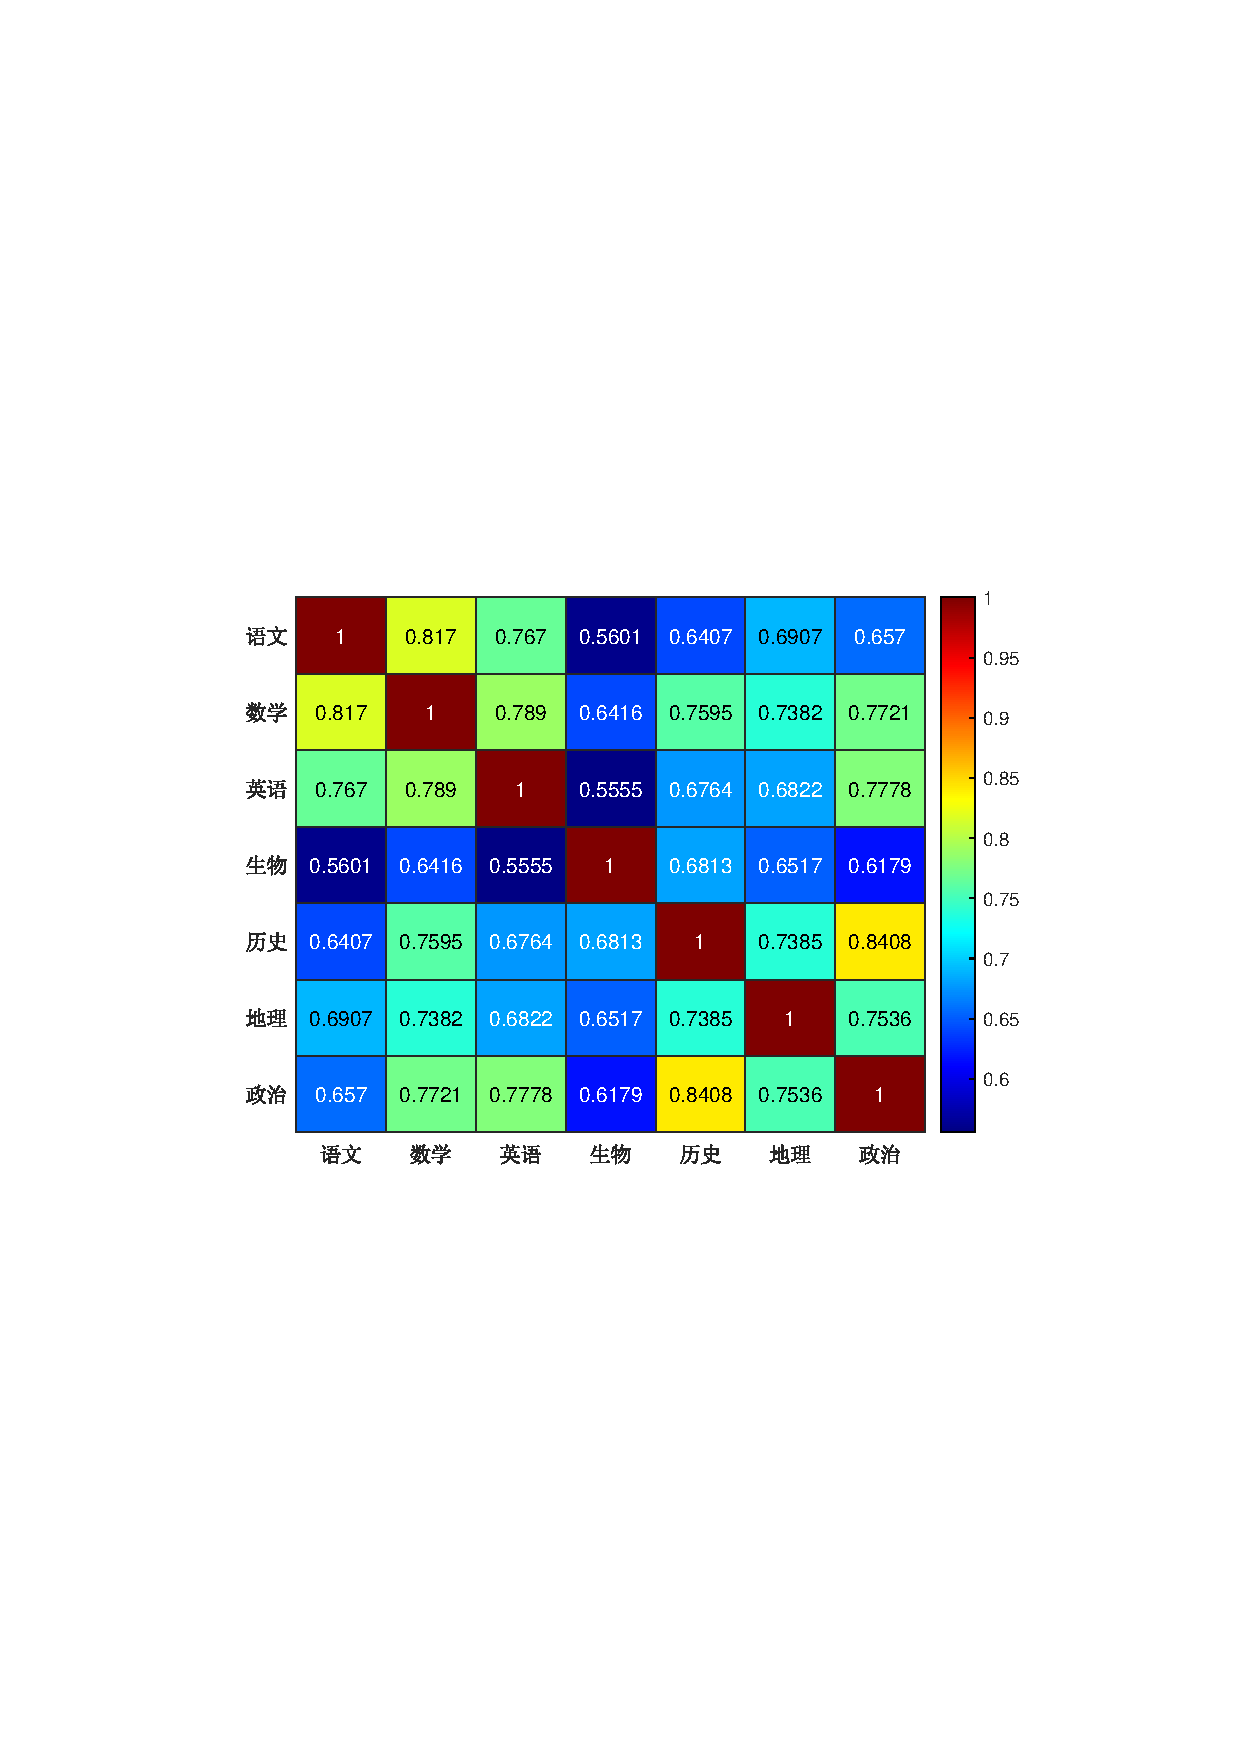
\includegraphics[width=0.8\textwidth]{相关系数热力图2}
    \caption{Spearman 相关系数热力图}
\end{figure}

Spearman 相关系数擅长于分析未知分布的定序变量数据。条件满足。

操作步骤和结果与 Pearson 相关系数类似。

\subsection{Kendall 相关系数}

\begin{table}[H]
    \centering
    \caption{Kendall 相关系数计算结果}\label{Tab:7}
    \begin{tabular}{|c|c|c|c|c|c|c|c|}
        \hline
           & 语文        & 数学        & 英语        & 生物        & 历史        & 地理        & 政治                  \\
        \hline
        语文 & 1.00(***) & 0.64(***) & 0.59(***) & 0.42(***) & 0.49(***) & 0.52(***) & 0.49(***) \bigstrut \\
        \hline
        数学 & 0.64(***) & 1.00(***) & 0.61(***) & 0.47(***) & 0.58(***) & 0.57(***) & 0.61(***) \bigstrut \\
        \hline
        英语 & 0.59(***) & 0.61(***) & 1.00(***) & 0.42(***) & 0.50(***) & 0.51(***) & 0.59(***) \bigstrut \\
        \hline
        生物 & 0.42(***) & 0.47(***) & 0.42(***) & 1.00(***) & 0.52(***) & 0.49(***) & 0.46(***) \bigstrut \\
        \hline
        历史 & 0.49(***) & 0.58(***) & 0.50(***) & 0.52(***) & 1.00(***) & 0.57(***) & 0.67(***) \bigstrut \\
        \hline
        地理 & 0.52(***) & 0.57(***) & 0.51(***) & 0.49(***) & 0.57(***) & 1.00(***) & 0.59(***) \bigstrut \\
        \hline
        政治 & 0.49(***) & 0.61(***) & 0.59(***) & 0.46(***) & 0.67(***) & 0.59(***) & 1.00(***) \bigstrut \\
        \hline
    \end{tabular}

    \vspace{0.3cm}
    {\zihao{5}注:***、**、*分别代表1\%、5\%、10\%的显著性水平}
\end{table}

\begin{figure}[H]
    \centering
    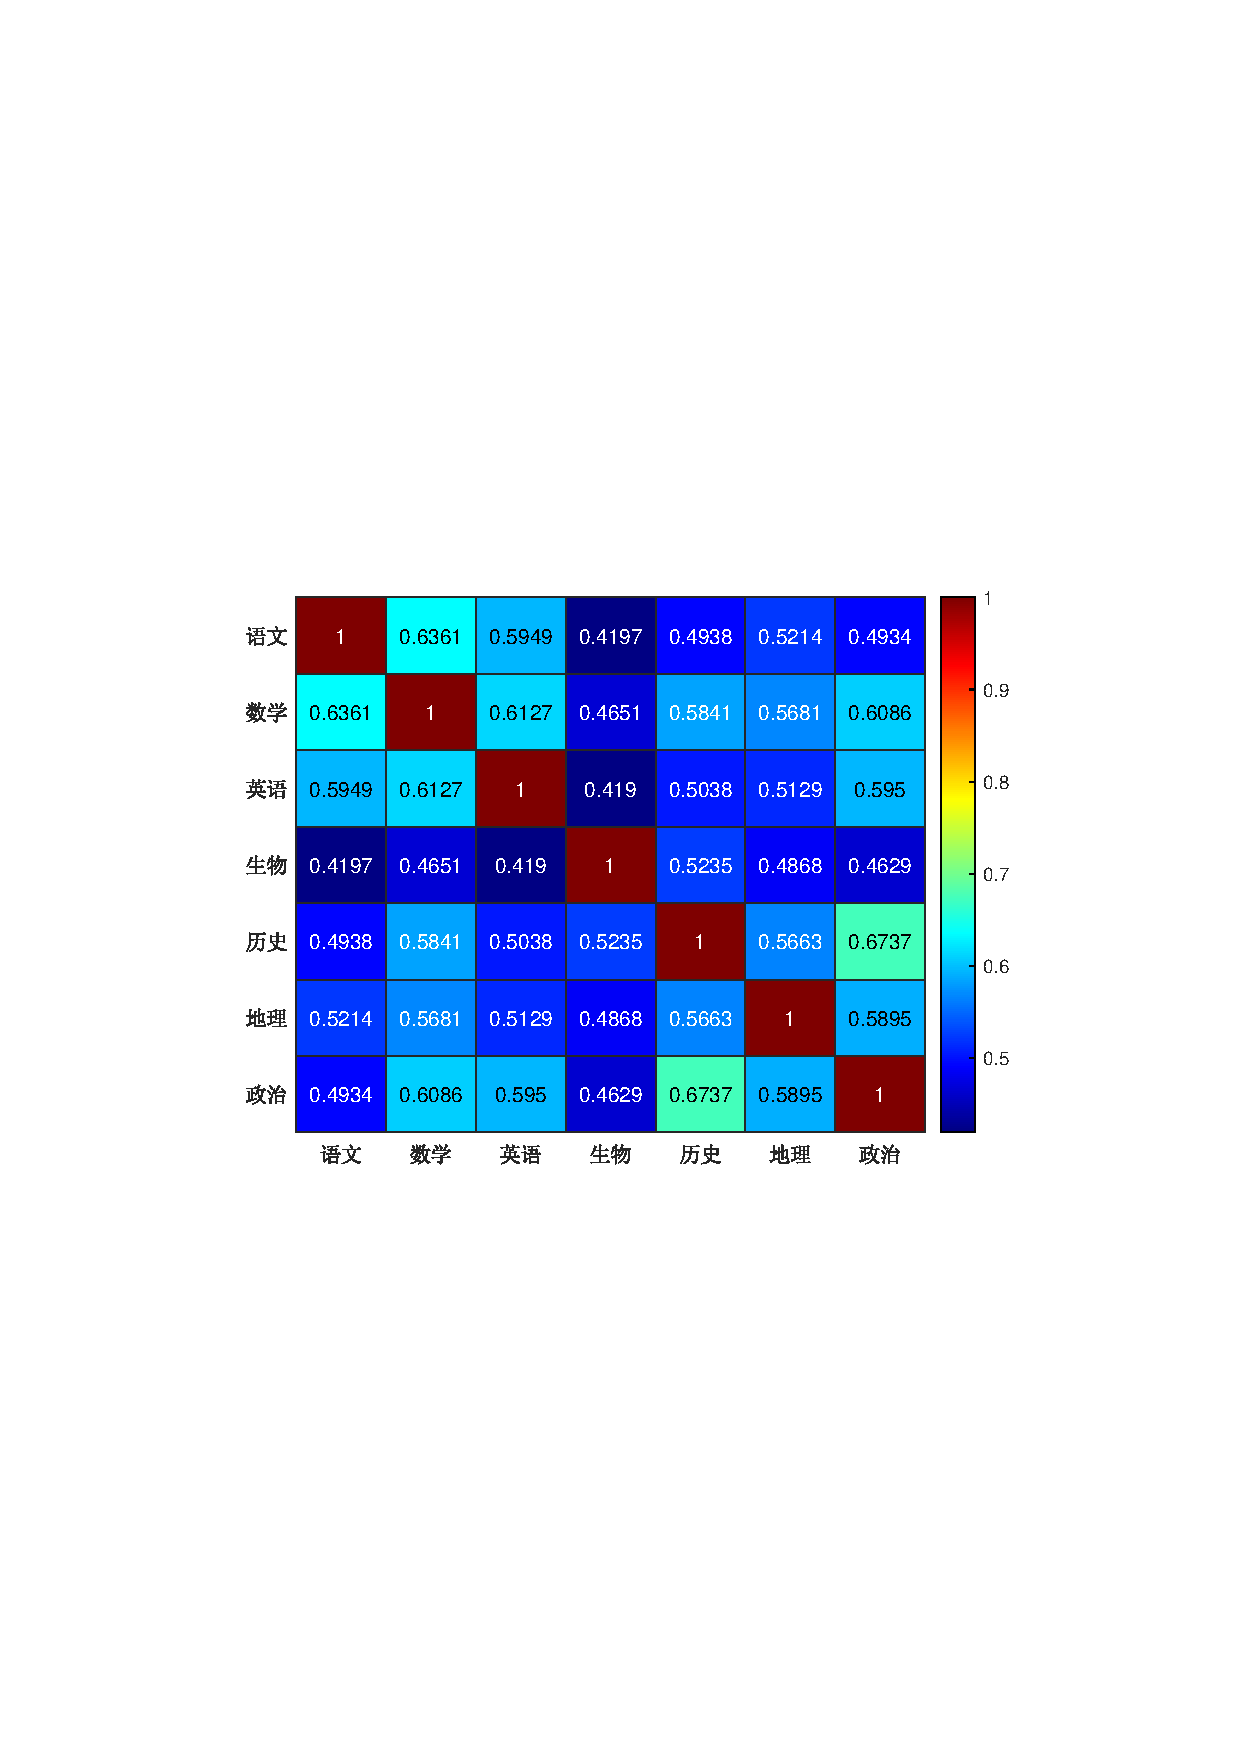
\includegraphics[width=0.8\textwidth]{相关系数热力图3}
    \caption{Kendall 相关系数热力图}
\end{figure}

Kendall 相关系数擅长于分析未知分布的定类和定序变量数据。条件满足。

操作步骤和结果与 Pearson 相关系数类似。

\appendix 

\section{Matlab 代码}
    \begin{lstlisting}[language=matlab ,caption={描述性统计} ]
    function result = DescriptiveStat(data)
    % 描述性统计
    % 各行分别为最大值,最小值,中位数,平均值,标准差,峰度,偏度
    Max = max(data);
    Min = min(data);
    Median = median(data);
    Mean = mean(data);
    Std = std(data);
    Kurt = kurtosis(data)-3;
    Skew = skewness(data);
    result = [Max;Min;Median;Mean;Std;Kurt;Skew];
    end
    \end{lstlisting}

    \begin{lstlisting}[language=matlab ,caption={相关系数分析示例} ]
    clc,clear

    %% 描述性统计
    data = readmatrix("data\相关系数示例.csv","NumHeaderLines",1);
    n = size(data,2);
    result = DescriptiveStat(data);
    disp(result);
    
    %% 绘制散点图矩阵
    figure(1);
    MatrixScatter(data);
    
    %% 绘制Q-Q图
    figure(2)
    for i=1:n
        subplot(2,4,i);
        qqplot(data(:,i));
        xlabel("");
        ylabel("");
        title("");
    end
    
    %% 正态性检验
    % Jarque-Bera 检验
    % jb_H = ones([n,1]);
    % jb_P = ones([n,1]);
    % for i=1:n
    %     [jb_h,jb_p] = jbtest(data(:,i),0.1);
    %     jb_H(i,1)=jb_h;
    %     jb_P(i,1)=jb_p;
    % end
    % disp([jb_H,jb_P]);
    
    % Shapiro-wilk 检验
    sw_H = ones([n,1]);
    sw_P = ones([n,1]);
    for i=1:n
        [sw_h,sw_p] = swtest(data(:,i),0.1);
        sw_H(i,1)=sw_h;
        sw_P(i,1)=sw_p;
    end
    disp([sw_H,sw_P]);
    
    %% 计算Pearson相关系数
    [Rp,Pp] = corrcoef(data);
    disp(Rp);
    disp(Pp);
    
    % 绘制相关系数热力图
    figure(3);
    names = ["语文","数学","英语","生物","历史","地理","政治"];
    heatmap(names,names,Rp);
    colormap("jet");
    
    %% 计算Spearman相关系数
    [Rs,Ps] = corr(data,"type","Spearman");
    disp(Rs);
    disp(Ps);
    
    % 绘制相关系数热力图
    figure(4);
    names = ["语文","数学","英语","生物","历史","地理","政治"];
    heatmap(names,names,Rs);
    colormap("jet");
    
    %% 计算Kendall相关系数
    [Rk,Pk] = corr(data,"type","Kendall");
    disp(Rk);
    disp(Pk);
    % 绘制相关系数热力图
    figure(5);
    names = ["语文","数学","英语","生物","历史","地理","政治"];
    heatmap(names,names,Rk);
    colormap("jet");        
    \end{lstlisting}

\section{Python 代码}

    \begin{lstlisting}[language=python ,caption=初始化 ]
    ## 导包
    import numpy as np
    import matplotlib.pyplot as plt
    import seaborn as sns
    import pandas as pd
    from scipy import stats
    import statsmodels.api as sm
    
    np.set_printoptions(suppress=True)
    
    plt.rcParams["font.sans-serif"] = ["SimHei"]  #设置字体
    plt.rcParams["axes.unicode_minus"] = False  # 解决图像中的“-”负号的乱码问题

    ## 数据初始化
    data = pd.read_csv("../data/相关系数示例.csv", encoding="gbk")
    n = data.shape[1]
    D = data.to_numpy()
    display(data)
    \end{lstlisting}

    \begin{lstlisting}[language=python ,caption={相关系数分析示例} ]
    ## 矩阵散点图
    for i in range(n):
    for j in range(n):
        plt.subplot(n, n, n * i + j + 1)
        plt.xticks([])
        plt.yticks([])
        if i != j:
            plt.scatter(D[:, i], D[:, j], 2)

    ## 描述性统计
    result0 = stats.describe(data)
    result = [result0.minmax[1], result0.minmax[0], data.median(), result0.mean, data.std(), result0.kurtosis,
            result0.skewness]
    result = pd.DataFrame(result, columns=data.columns,
                        index=["最大值", "最小值", "中位数", "平均值", "标准差", "峰度", "偏度"])
    display(result)

    ## Pearson相关系数
    # Q-Q图
    plt.figure(figsize=(10, 5))
    for i in range(n):
        sub_ax = plt.subplot(2, 4, i + 1)
        sm.qqplot(D[:, i], ax=sub_ax, line='45', fit=True, markersize=4, marker="x")
        sub_ax.set_xlabel(None)
        sub_ax.set_ylabel(None)
        sub_ax.set_xticks([])
        sub_ax.set_yticks([])
        plt.subplots_adjust(wspace=0.1, hspace=0.1)

    # 正态性检验
    #jbtest_result = []
    #for i in range(n):
        #jb, jb_p = stats.jarque_bera(D[:, i])
        #jbtest_result.append([jb, jb_p])
    #jbtest_result = pd.DataFrame(jbtest_result, columns=["jb值", "p值"], index=data.columns)
    #display(jbtest_result)
    swtest_result = []
    for i in range(n):
        W, sw_p = stats.shapiro(D[:, i])
        swtest_result.append([W, sw_p])
    swtest_result = pd.DataFrame(swtest_result, columns=["W值", "p值"], index=data.columns)
    display(swtest_result)

    # 相关系数计算
    Rp = np.ones((n, n))
    Pp = np.ones((n, n))
    for i in range(n):
        for j in range(n):
            rp, pp = stats.pearsonr(D[:, i], D[:, j])
            Rp[i, j] = rp
            Pp[i, j] = pp
    Rp = pd.DataFrame(Rp, columns=data.columns, index=data.columns)
    Pp = pd.DataFrame(Pp, columns=data.columns, index=data.columns)
    display(Rp)
    display(Pp)

    # 热力图
    sns.heatmap(Rp, xticklabels=data.columns, yticklabels=data.columns, annot=True, cmap="jet", fmt=".4f")
    plt.show()

    ## Spearman相关系数

    # 相关系数计算
    Rs = np.ones((n, n))
    Ps = np.ones((n, n))
    for i in range(n):
        for j in range(n):
            rs, ps = stats.spearmanr(D[:, i], D[:, j])
            Rs[i, j] = rs
            Ps[i, j] = ps
    Rs = pd.DataFrame(Rs, columns=data.columns, index=data.columns)
    Ps = pd.DataFrame(Ps, columns=data.columns, index=data.columns)
    display(Rs)
    display(Ps)

    # 热力图
    sns.heatmap(Rs, xticklabels=data.columns, yticklabels=data.columns, annot=True, cmap="jet", fmt=".4f")
    plt.show()

    ## Kendall 相关系数

    # 相关系数计算
    Rk = np.ones((n, n))
    Pk = np.ones((n, n))
    for i in range(n):
        for j in range(n):
            rk, pk = stats.kendalltau(D[:, i], D[:, j])
            Rk[i, j] = rk
            Pk[i, j] = pk
    Rk = pd.DataFrame(Rk, columns=data.columns, index=data.columns)
    Pk = pd.DataFrame(Pk, columns=data.columns, index=data.columns)
    display(Rk)
    display(Pk)

    # 热力图
    sns.heatmap(Rk, xticklabels=data.columns, yticklabels=data.columns, annot=True, cmap="jet", fmt=".4f")
    plt.show()
    \end{lstlisting}
    
\end{document}